\section{A Data Set for Camera-Independent Color Constancy}

\begin{flushleft}
    \author{
    Ça$ \breve{g} $lar Aytekin, 
    Jarno Nikkanen, 
    Moncef Gabbouj
    \emph{Fellow, IEEE}
    }
\end{flushleft}

\begin{center}
    \emph{IEEE TRANSACTIONS ON IMAGE PROCESSING, VOL. 27, NO. 2, FEBRUARY 2018}
\end{center}

\subsection{INTRODUCTION}
Color constancy is a characteristic of the human visual system (HVS) that 
helps to perceive a constant color, for example of an object, at different levels 
of illuminations. It is claimed that the achievement of constancy occurs by 
approximating the composition of the lighting in order to obtain the true 
color of the object. There are supervised and unsupervised methods 
that calculate color consistency. Unsupervised methods are divided into two 
categories, based on the techniques they use to estimate the color of 
the illuminating source. The first category makes statistical assumptions 
about reflectance in a scene. The second category instead uses the physical 
properties of objects in scenes. Supervised methods also fall into two categories. 
The first category tries to learn a combination of unsupervised methods to 
estimate the illumination. The second category builds its own model for 
learning about illumination. The major factor affecting all of these methods 
is the sensitivity of the camera sensor. When the sets used for training, 
validation and testing contain images taken by different cameras, the results 
returned by the algorithms may be different, as well as their performance. 
On the other hand, one method returns "fixed" results when operating on 
images from the same camera. In the CC field, this problem is called camera-independence.
This report provides a dataset, called \emph{Intel-TUT}, which is 
useful for testing camera-independence in the CC. Three different cameras 
capture real scenes both in the lab and elsewhere. Laboratory images have 
different lighting conditions. The dataset contains 1536 images and a test 
set consisting of 454 images taken by a single camera.

\subsection{COLOR CONSTANCY DATASETS}
One of the first datasets for calculating the CC was the one proposed in 
\cite{0807099130}. The single camera captured images showing a total of 1995 surfaces, 
11 lab illuminations and 81 illuminations from the real world. The dataset 
also contains a number of images that make up 50 scenes. After a correct 
calibration, it removes the irrelevant images, the remainder was made up of 
only 529 images which made up 30 scenes. Each of these images belongs to 
the set captured in the lab. Another dataset is the one proposed in \cite{0807099132}, consisting 
of 11,000 images of indoor / outdoor scenes. The scenes were captured in 
different geographic locations and under different weather conditions. Unfortunately 
this dataset contains low resolution images that require a correction 
phase. Another dataset containing 246 indoor images and 322 outdoor images, 
taken by two different cameras, is the one proposed in \cite{0807099120}. Another 
dataset that uses the auto-bracketing technique to acquire the images is the 
one proposed in \cite{0807099134}. In this dataset they are acquired up to 9 different 
images, of the same scene, with different settings for each shot. A dataset that 
aims to obtain multiple lighting in a scene is the one proposed in \cite{0807099135}. 
This contains relatively few images, 9 acquired in an outdoor environment 
and 59 lab images. The is also a dataset containing the videos mentioned 
in \cite{0807099136}. There was only one study \cite{0807099129} that relies on color conversion in order 
to achieve camera independence. However, this method requires a very 
sensitive spectral camera to achieve good performance, so it is not applicable 
to all images. Finally, a last dataset consisting of 1600 indoor and outdoor 
images, taken by 9 different cameras, is the one proposed in \cite{0807099128} called NUS. 
In this collection, each scene was captured by each camera with slight misalignments. 
The database proposed in this paper is similar to the NUT only 
for the different cameras used. However, the proposed database has some 
features such as the following:
\begin{itemize}
    \item Provides the spectral sensitivities of the cameras;
    \item Different illuminants illuminate the scene;
    \item Among the different cameras used, one is mobile;
    \item Provides a set of tests for good evaluation of CC methods.
\end{itemize}

\subsection{THE PROPOSED INTEL-TUT DATA SET}
The purpose of the dataset is to help the algorithms to determine if the color 
constancy value obtained is to be considered good or not. If an algorithm 
does not find a change in this value on the same set of images taken by the 
same camera, then this algorithm is able to have a uniform color constancy 
and consequently would produce optimal outputs. Each image in the 
dataset has undergone several changes such as: black level correction (BLC), 
color shading correction (CSC) (only for mobile camera), white balance (WB), 
color conversion from RGB sensor to sRGB (CCM) , gamma correction of 
0.45, sharpening effect correction (blur) and brightness normalization.

\subsubsection{Light Sources}
A variety of devices were used that were capable of producing a light source. 
Each property such as luminance (Lux), color temperature (CCT) and CIE 
xy chromaticity, have been appropriately set to have an equitable acquisition.

\subsubsection{Cameras}
Three types of camera are used for the construction of the dataset. Two 
of these belong to the high-end, while a third belongs to the category of 
mobile. To achieve correct color correction, several 3x3 size color 
conversion matrices (\emph{CCMs}) were used. In other words, try to transform 
the components of the image from RGB to sRGB in order to adapt them to 
the lighting under which the image is viewed. For the outdoors, 10 CCMs 
were used based on the type of illumination. Another factor that required 
correction was the color shading (\emph{CS}). This only requires correction for the 
images coming from the mobile.

\subsubsection{Scene Contents}
The scenes that make up the dataset are divided into lab scenes and field 
scenes. There are several types of different lab scenes, each having 5 different 
illuminations (Fig. \ref{fig:Lab}). Both the lab scenes and those acquired in the field 
are 64, for a total of 128 scenes. Each lab scene is captured with each camera 
in almost the same shot. An attempt was made to preserve the same settings 
in the field scenes even if the latter have different lighting. In order to have 
good stabilization, a fixed tripod is used.
\begin{figure}[htbp]
    \centering
    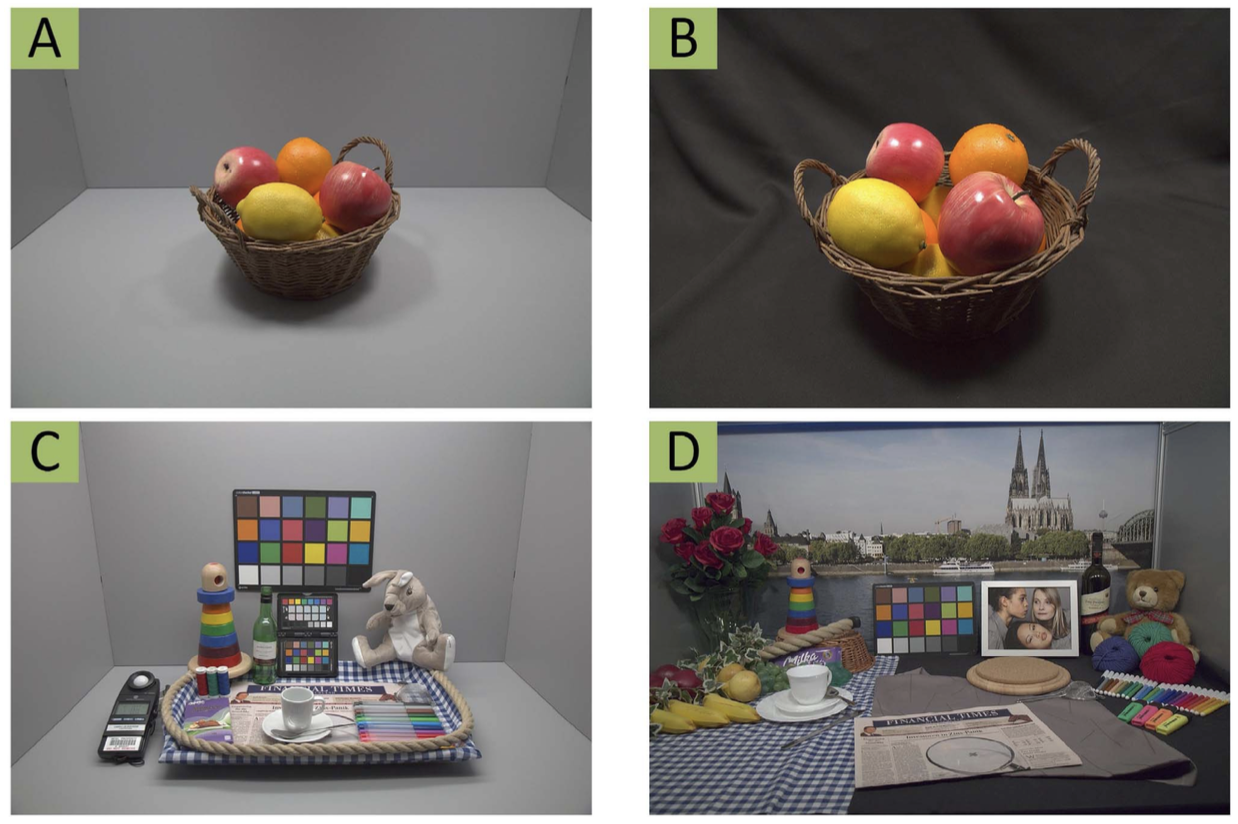
\includegraphics[width = 0.6 \linewidth]{images/paper4/lab.png}
    \centering
    \caption{Lab real scenes}
    \label{fig:Lab}
\end{figure}

\subsubsection{Ground Truths}
The ground-truth is based on the chromaticity of the illumination, or white 
points, assumed by the camera which can change for each image. This parameter 
is calculated by averaging the achromatic colors present in the lighter 
patches of the color-checker, that appear in the last line.

\subsubsection{Recommendations for Evaluating CC Algorithm Performance}\label{recommend}
In order to evaluate the performance of the algorithm with this type of 
dataset, it is recommended to use the following strategies:
\begin{enumerate}
    \item \emph{Camera independence}: the article proposes six-fold cross validation, 
    where each fold, divided into training, validation and test, contains a 
    grouping of images for each of the nine cameras. This technique aims 
    to obtain a fair evaluation of camera-independence of an algorithm (the 
    algorithm considers all images as if coming from the same camera).
    \item \emph{Camera and Scene Independence}: in this case it is recommended to 
    use the images acquired by Nikon and the mobile for training, while 
    the Canon images must be used for validation. As for the test, it is 
    recommended to use the Canon images belonging to the second group 
    of images. In this way you can understand the influence of camera-
    independence. If you get a low error, which means that the algorithm 
    treats each scene (each made up of images captured by different cameras) 
    as if it had been captured entirely by a single camera, then at 
    this point you would get, in addition to independence of the camera, 
    the independence of the scene. This is a good result if it is achieved in 
    this type of dataset.
    \item \emph{Camera and Scene Independence from Single Camera}: in this strategy 
    it is suggested to use the images from the second group as training 
    and validation while using the images acquired by Nikon and the 
    mobile for testing. In this way we want to understand if the algorithm 
    obtains the camera/scene independence effect with images produced 
    by another different camera (Canon). If this technique were 
    used with the 1 (where a low error implies the achievement of the 
    camera-independence) then when new images of different origin would 
    be inserted, the error would be higher than that obtained in 1, this is 
    because the camera-independence it faces the old set of cameras and not 
    the new one. It is being said that thanks to the combination of these, 
    it is possible to have a targeted camera-independence and a targeted 
    scene-independence for each new camera.
    \item \emph{Testing the Effect of Color Shading}: if you were to use the images 
    of your mobile, to test their color shading correction (CS), you could 
    enclose them all in a test set. Images that cause a high error will be 
    those that have not undergone the correction process.
    \item \emph{Testing the Effect of Resolution}: color constancy can be easily calculated 
    when the images are at high resolution. As you can guess, this 
    result is not achievable with images from a mobile phone. For this 
    reason, the dataset contains a portion of image downscaling (1080p) 
    useful for observing how the resolution can affect the performance of 
    the algorithm.
\end{enumerate}

\subsection{EXPERIMENTAL RESULTS}
\subsubsection{Evaluation of Unsupervised Baseline Methods}
In summary, in order to have the effect of the camera-independecy on a 
set of images from different cameras, it is enough to be able to calculate 
the constancy of the color which, in other words, means having to detect the 
chromaticity of the illuminate that precisely illuminates the scene. Given the 
chromaticity estimated by the algorithm ($ p^{Est} $) and the effective chromaticity 
(white point or ground truth) ($ p^E $), the performance of an algorithm can be 
evaluated based on the result returned by the recovery angular error (RAE):
\begin{equation}
    RAE=\cos^{-1}\left(\frac{p^Ep^{Est}}{||p^E||~||p^{Est}||}\right)
\end{equation}
This error index is calculated both on the performances obtained in high 
resolution images and in those obtained at low resolution. To make some 
comparison, an algorithm that has a low RAE is the unsupervised algorithm 
GW \cite{0807099104} which assumes that the average chromaticity in an image is gray. 
Even the MaxRGB algorithm \cite{0807099103} manages to have good performance 
in images where there are saturated areas where, thanks to these, the white 
point can be easily recovered. MaxRGB is currently the only algorithm that 
manages to have a low RAE even with low quality images (1080p). The 
performances of these algorithms, together with two others (SoG and GE), 
are compared in figure \ref{fig:RAE} where for each set of images (Lab 
Printouts, Lab Real Scenes, $ 1^{st} $ Field Set and $ 2^{nd} $ Field set), taken from different cameras, 
are calculated mean, median and maximum of RAE values reached for each 
image. Subsequently, in figure \ref{fig:RAEstandard} the mean, median and maximum of the 
standard deviation obtained from each image, from each algorithm, are calculated 
again. As you can see, the GW algorithm is the only one to have the 
camera-independence for all the rooms used.

\begin{figure}[htbp]
    \centering
    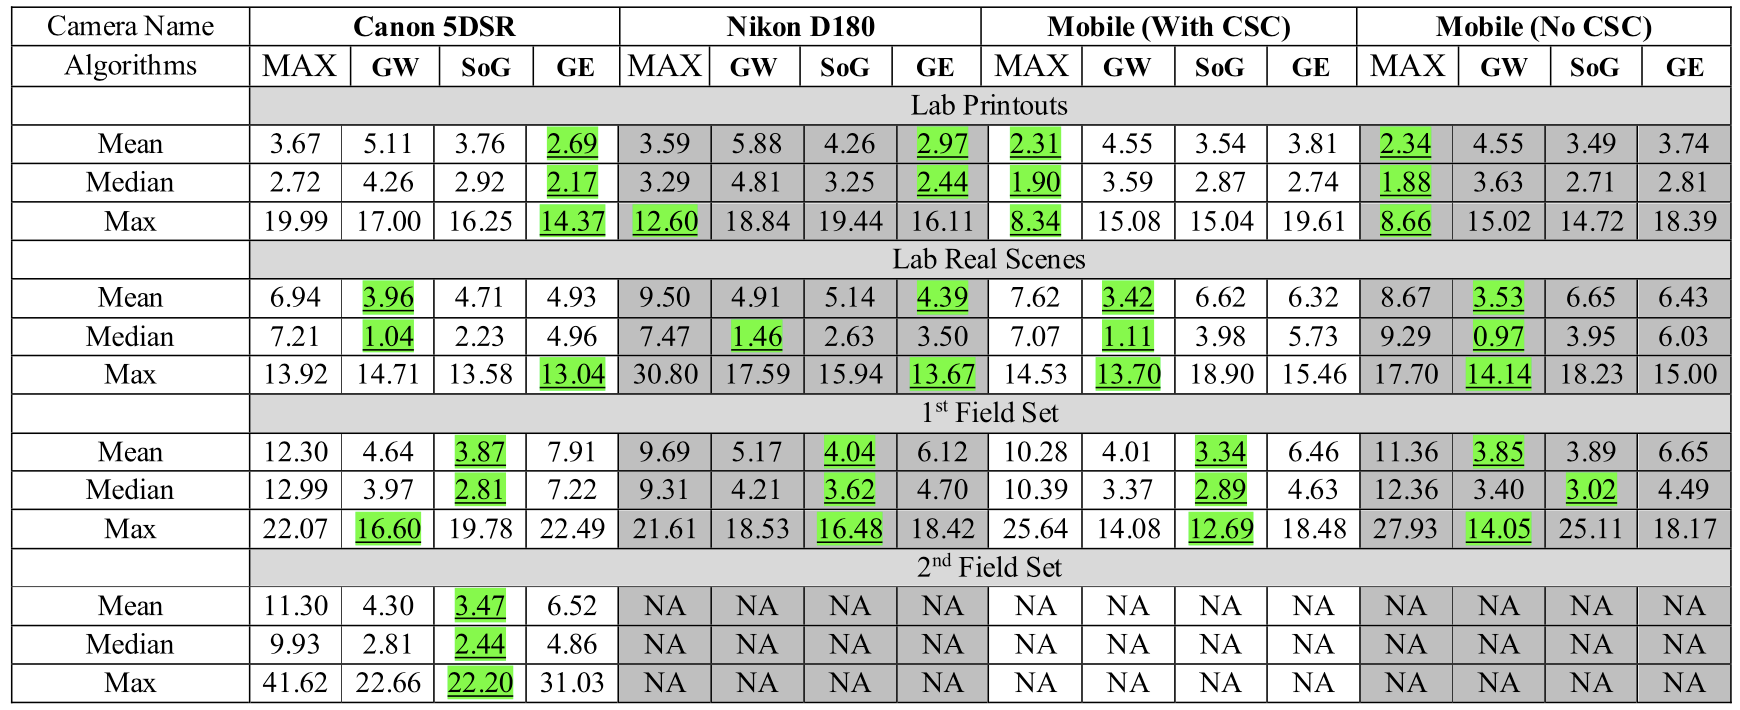
\includegraphics[width = 1 \linewidth]{images/paper4/RAEHigh.png}
    \centering
    \caption{Recovery Angular Errors (Mean, Median and Maximum) of some algorithms.}
    \label{fig:RAE}
\end{figure}

\begin{figure}[htbp]
    \centering
    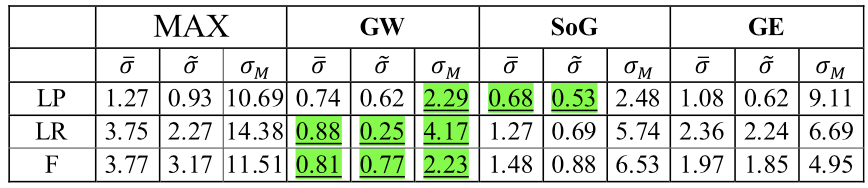
\includegraphics[width = 0.6 \linewidth]{images/paper4/standardHigh.png}
    \centering
    \caption{Mean, Median and Maximum RAE of some algorithms.}
    \label{fig:RAEstandard}
\end{figure}

\subsubsection{Evaluation of a Direct Supervised Method}
In order to be able to calculate color constancy, and thus be able to achieve 
the camera-independence, various methods were used that included the use 
of convolutional neural networks (CNNs). In method \cite{0807099122}, the network used 
is composed of a convolutional layer with 240 filters of size 1x1, the usual 
function of ReLU, a max-Pooling of blocks of size 8x8 with stride 8. Finally 
there is a fully-connected layer with 40 layers hidden and a 3-dimensional 
output in which there is the estimated chromaticity of the lighting. In order to demonstrate the validity of the proposed dataset, the use of CNN has been adapted to the techniques described in \ref{recommend}:
\begin{enumerate}
    \item Following technique 1, various CNNs are trained to provide the least 
    possible error. The error reached by the model is less than when using 
    the Canon for training and validation. This means that the networks 
    assume the camera-independence only with the Nikon and mobile models. 
    Therefore the networks would be able to recognize new cameras. As 
    can be seen in the figure, the RAE values between the various cameras 
    are very similar (Fig. \ref{fig:CNNtec1}).
    \begin{figure}[htbp]
        \centering
        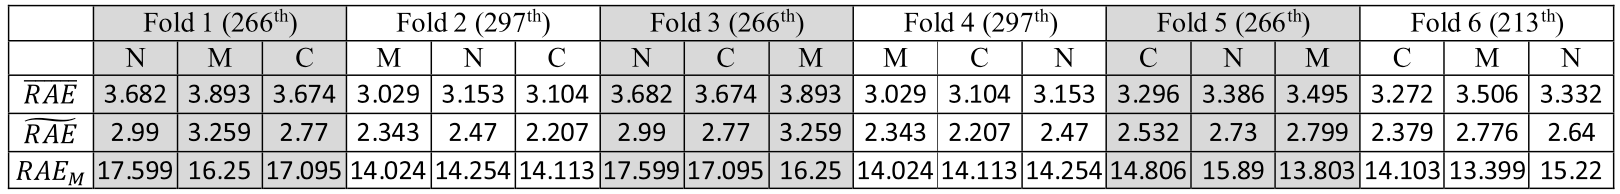
\includegraphics[width = 1 \linewidth]{images/paper4/CNNtec1.png}
        \centering
        \caption{Camera Independence of \cite{0807099122} with CCM on $ 1^{st} $ thecnique. Mean, Median and Maximum RAE of CNN.}
        \label{fig:CNNtec1}
    \end{figure}
    \item Now a CNN is trained using technique 2. The training is carried out 
    with images acquired from both Nikon and mobile. Canon's images are 
    used for validation, while Canon's images belonging to the $ 2^{nd} $ field 
    are used for the test. Low errors are obtained with the use of a color 
    conversion matrix (CCM) \cite{0807099129} and therefore the model manages to have 
    the camera/scene-independence (Fig. \ref{fig:CNNtec2}).
    \begin{figure}[h!]
        \centering
        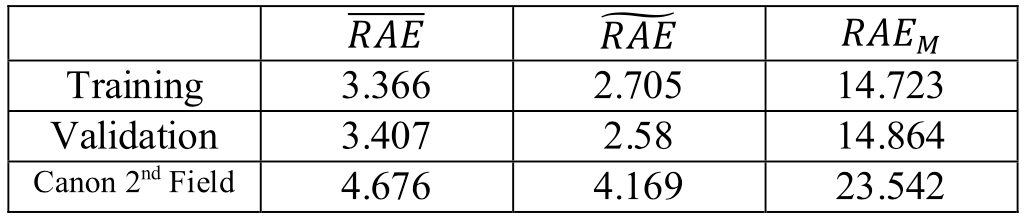
\includegraphics[width = 0.6 \linewidth]{images/paper4/CNNtec2.png}
        \centering
        \caption{Camera Independence of \cite{0807099122} with CCM on $ 2^{nd} $ thecnique. Mean, Median and Maximum RAE of CNN.}
        \label{fig:CNNtec2}
    \end{figure}
    \item According to technique 3, a CNN can be trained to reach camera independence 
    only on one camera, excluding the others. In this case, since 
    the images of the $ 2^{nd} $ field, used for both training and validation, belong 
    only to Canon, then CNN will get the camera/scene-independence 
    only on this type of camera (Fig. \ref{fig:CNNtec3}).
    \begin{figure}[h!]
        \centering
        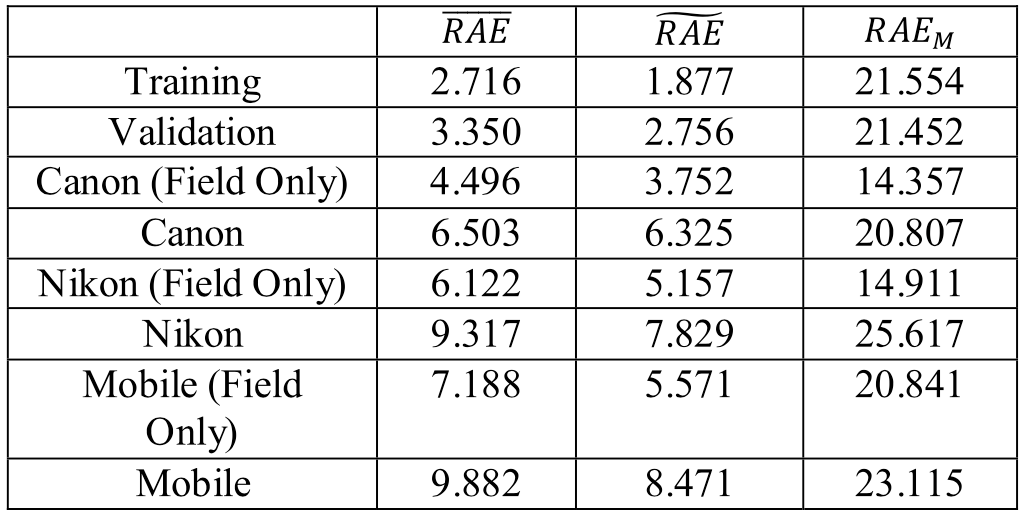
\includegraphics[width = 0.6 \linewidth]{images/paper4/CNNtec3.png}
        \centering
        \caption{Camera Independence of \cite{0807099122} on $ 3^{nd} $ thecnique. Mean, Median and Maximum RAE of CNN.}
        \label{fig:CNNtec3}
    \end{figure}
\end{enumerate}

\subsubsection{A State of the Art Camera Independent Method}
The following section presents a competitive method \cite{0807099125} that can beat the 
performance of \cite{0807099122}. Also in this new method there is an even deeper CNN 
that uses a set of images on which a CCM pre-processing phase has already 
been applied. The comparisons of the results obtained by \cite{0807099122} and by \cite{0807099125} in 
all the techniques proposed in \ref{recommend} where it can be seen that all the error 
rates of \cite{0807099125} are smaller than those of \cite{0807099122} and therefore the model is able to 
reach the camera/scene-independece more easily.
\begin{figure}[htbp]
    \centering
    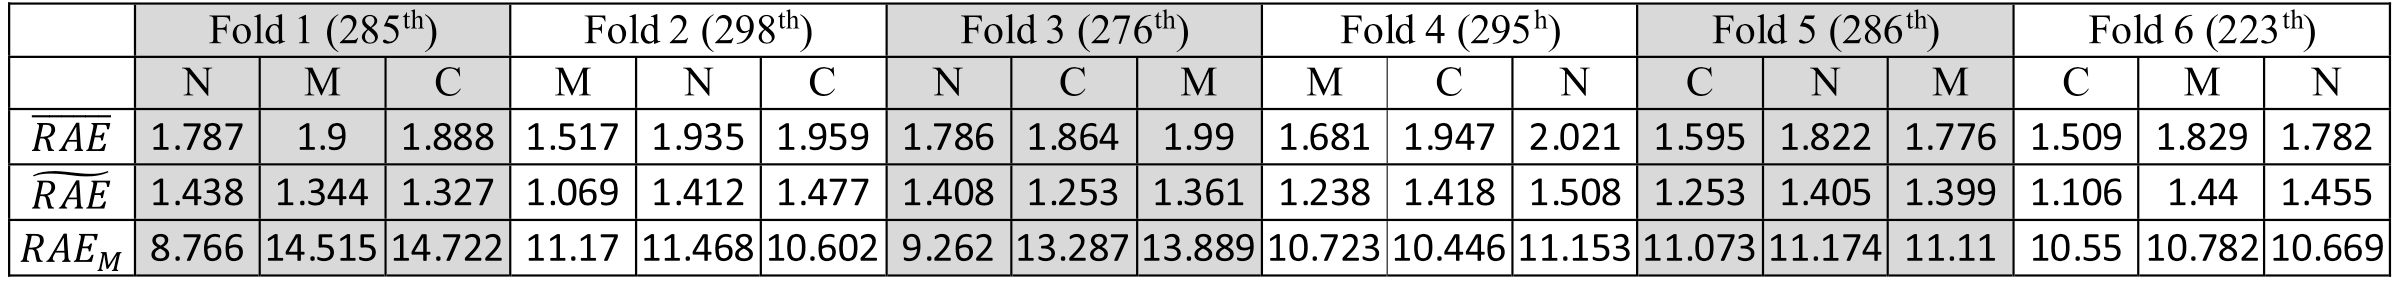
\includegraphics[width = 1 \linewidth]{images/paper4/25tech1.png}
    \centering
    \caption{Camera Independence of \cite{0807099122} with CCM on $ 1^{nd} $ thecnique. Mean, Median and Maximum RAE of CNN.}
    \label{fig:25t1}
    \begin{minipage}[t]{.45\linewidth}
        \centering
        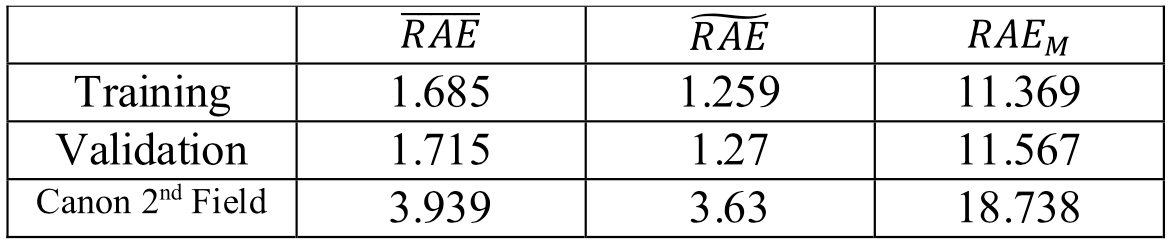
\includegraphics[width=\linewidth]{images/paper4/25tech2.png}
        \caption{\small Camera Independence of \cite{0807099122} on $ 2^{nd} $ thecnique. Mean, Median and Maximum RAE of CNN.}\label{fig:1}
    \end{minipage}
    \hfill
    \begin{minipage}{.45\linewidth}
        \centering
        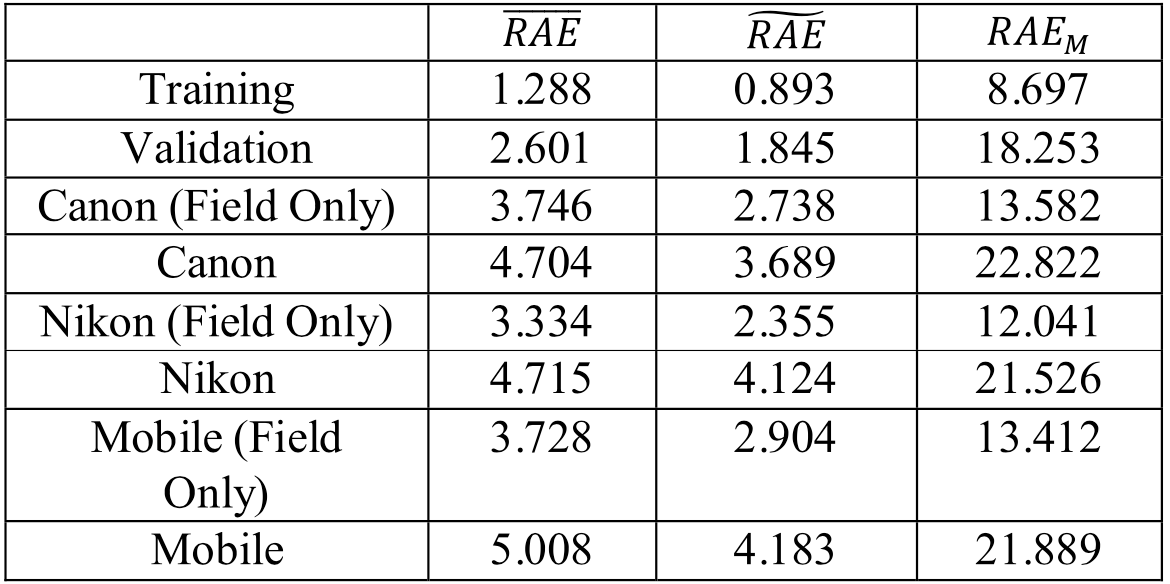
\includegraphics[width=\linewidth]{images/paper4/25tech3.png}
        \caption{\small Camera Independence of \cite{0807099122} on $ 3^{nd} $ thecnique. Mean, Median and Maximum RAE of CNN.}\label{fig:1}
    \end{minipage}  
    \label{fig:1-2}
\end{figure}

\subsection{CONCLUSION}
The dataset proposed in this paper is useful for testing the behavior of 
an algorithm, or a model based on CNN, in the search of camera/scene-independece. 
If the algorithm manages to obtain this benefit, then it will be 
able to generalize a scene composed of several images acquired from different 
cameras, otherwise the results returned by this will be highly variable. 
Achieving this goal can also be done using a CNN if the CMM process is 
applied to its input set. It is necessary to specify that, in order to 
achieve the final result, it is essential to have the spectral sensitivities of each camera 
without which it would not be possible to achieve camera independence.